\documentclass[12pt,a4paper]{article}

% =========================
% Packages
% =========================
\usepackage[utf8]{inputenc}
\usepackage[T1]{fontenc}
\usepackage[ngerman]{babel}
\usepackage[a4paper,margin=2.5cm]{geometry}
\usepackage{setspace}
\usepackage{csquotes}
\usepackage[hidelinks]{hyperref}
\usepackage{graphicx}
\usepackage{booktabs}
\usepackage{amsmath,amssymb}

\onehalfspacing

% =========================
% Bibliography
% =========================
\usepackage[
  backend=biber,
  style=alphabetic,
  sorting=nyt
]{biblatex}

\addbibresource{references.bib}

% =========================
% Title
% =========================
\title{
  LLM Prompt Injection Defences\\
  \large Strukturierte Anfragen und Grenzen aktueller Schutzmechanismen
}

\author{
  Denis Krüger \\
  Sebastian Mautner\\
  Technische Hochschule Würzburg-Schweinfurt \\
   SS 2026
}
\date{}
% =========================
% Document
% =========================
\begin{document}

\maketitle

\begin{abstract}
Diese Arbeit untersucht Prompt Injection als Sicherheitsproblem in LLM-integrierten Anwendungen.
Im Fokus stehen Angriffsmodelle, Verteidigungsansätze sowie deren Grenzen.
Besonderes Augenmerk liegt auf der Trennung von Instruktionen und Daten als Verteidigungsstrategie.
\end{abstract}

\tableofcontents
\newpage

\section{Introduction}
\label{sec:einleitung}

Large Language Models (LLMs) are increasingly integrated into applications that
read emails, summarise documents, retrieve web content, and execute actions on
behalf of users. This increases their usefulness but also exposes them to
content controlled by parties other than the application operator.

Prompt injection exploits this exposure by placing malicious instructions in
content processed by the model. If the model follows the injected instruction
instead of the trusted task, it may manipulate a response, disclose protected
information, or influence a connected tool
\parencites{perez2022ignore}{greshake2023indirect}. The 2025 OWASP Top 10 for
LLM Applications assigns prompt injection the identifier \emph{LLM01}, marking
it as the first category listed in the document
\parencite{owasp2025llm}.

Applications can encode developer instructions, user input, and tool results
using different roles or delimiters. These distinctions influence model
behaviour, but they do not constitute access control. Unlike a prepared SQL
statement, a prompt format does not give natural-language text a reliably
enforced type or authority. Security cannot therefore rely on formatting alone
to preserve the distinction between trusted instructions and untrusted data
\parencites{liu2023promptinjection}{wallace2024instruction}.

StruQ and SecAlign address this problem by training models to maintain an
instruction--data separation. Their original evaluations report substantial
reductions in attack success, particularly against manually constructed attacks
\parencites{chen2025struq}{chen2025secalign}. However, reported robustness is
difficult to compare across studies because evaluations differ in models,
tasks, attacker access, optimisation methods, and success criteria. Later
defence-adaptive studies further question whether results obtained under narrow
attack suites generalise to stronger attacker models
\parencites{jia2025critical}
             {yang2025checkpointgcg}
             {pandya2025astra}.

This creates two related questions: how much security can learned
instruction--data separation provide under the evaluated conditions, and how
should applications limit the consequences when the model still follows an
injected instruction?

\medskip
\noindent\textbf{Research Question} \quad
\textit{How effectively do learned instruction--data separation approaches
mitigate prompt injection under the evaluated attacker models, and what
system-level controls are required when they do not provide an independently
enforced security boundary?}

\medskip
To answer this question, the paper compares the original StruQ and SecAlign
evaluations with later defence-adaptive studies and relates their limitations
to system-level security controls. No original experiments or independent
replications are conducted.

Chapter~\ref{sec:llms} introduces LLM prompting and structured context.
Chapter~\ref{sec:prompt-injection} describes prompt-injection delivery and
construction methods, and Chapter~\ref{sec:threat} defines the threat model used
for the comparison. Chapter~\ref{sec:struq} examines StruQ and SecAlign, while
Chapter~\ref{sec:limits} evaluates the limits of their reported robustness.
Chapter~7 derives practical deployment implications, and
Chapter~\ref{sec:conclusion} answers the research question.
\section{LLMs and Prompting}
\label{sec:llms}

Large Language Models are typically pretrained to predict tokens conditioned on
preceding context. This objective supports general-purpose instruction following
after further training, enabling tasks such as summarisation, translation,
question answering, and code generation
\parencites{brown2020language}{chen2025struq}.

In an LLM-integrated application, the model may receive application-provided
higher-priority instructions, a user request, retrieved data, and tool results.
Interfaces normally encode these components using role markers or delimiters,
and instruction-hierarchy training can teach a model to prioritise some channels
over others
\parencite{wallace2024instruction}. These distinctions are meaningful inputs to
the model. They do not, however, constitute an independently enforced authority
mechanism: generation still depends on learned behaviour over the combined
context.

Prompt injection exploits failures of that learned prioritisation. An attacker
crafts text in an untrusted channel so that the model treats it as a controlling
instruction rather than as task-relevant data
\parencite{liu2023promptinjection}. Structured prompting can make the intended
roles clearer and model training can improve adherence to them, but downstream
security should not assume that formatting alone prevents untrusted text from
influencing generation.

\section{Prompt Injection Attacks}
\label{sec:prompt-injection}

Prompt injection occurs when attacker-controlled text is interpreted as an
instruction that overrides or redirects the trusted task
\parencite{perez2022ignore}. This does not necessarily require a conventional
software defect. The failure arises because an instruction-following model can
assign authority to text from an unintended source. The surrounding application
turns that behavioural failure into a security problem when it exposes protected
data or permits consequential actions.

\subsection{Direct and Indirect Prompt Injection}

The literature distinguishes two principal delivery mechanisms
\parencite{greshake2023indirect}.

In a \emph{direct prompt injection}, a malicious user submits the payload through
the target application's ordinary user-input channel. The attacker may ask the
model to ignore the established task, imitate a higher-priority instruction, or
begin a new task
\parencite{perez2022ignore}. Figure~\ref{fig:direct-prompt-injection} shows both
the trusted instruction and the competing attacker-controlled input.

\begin{figure}[htbp]
    \centering
    \begin{tikzpicture}[
        box/.style={draw, rounded corners, align=center, text width=2.5cm,
                    minimum height=0.9cm},
        untrusted/.style={box, dashed},
        flow/.style={-{Latex[length=2.2mm]}, thick}
    ]
        \node[box] (trusted) at (1.4,1.3)
            {Trusted application\\instruction};
        \node[untrusted] (attacker) at (1.4,-1.3)
            {Malicious user's\\direct input};
        \node[box] (application) at (5.0,0)
            {Application\\prompt construction};
        \node[box] (llm) at (8.7,0)
            {Large Language\\Model};
        \node[box] (output) at (12.4,0)
            {Model\\output};

        \draw[flow] (trusted) -- (application);
        \draw[flow] (attacker) -- (application);
        \draw[flow] (application) -- (llm);
        \draw[flow] (llm) -- (output);
    \end{tikzpicture}
    \caption[Direct prompt injection]{Direct prompt injection through the
    application's user-input channel. The malicious input is combined with the
    trusted application instruction during prompt construction. Original
    schematic based on \textcite{perez2022ignore}.}
    \label{fig:direct-prompt-injection}
\end{figure}

In an \emph{indirect prompt injection}, the payload is delivered through content
that the application retrieves or receives during normal operation, such as a
web page, document, email, application programming interface (API) response, or
tool output. The attacker need not submit the completed payload directly to the
target application. This makes indirect injection comparatively covert, but not
inherently more damaging: the impact still depends on the data and authority
available to the application
\parencites{greshake2023indirect}{debenedetti2024agentdojo}.

Retrieval-augmented generation (RAG) systems and tool-using agents are exposed
because they routinely place external content in the model context. As
Figure~\ref{fig:indirect-prompt-injection} illustrates, trusted and untrusted
inputs converge at the application even though they originate from different
principals.

\begin{figure}[htbp]
    \centering
    \begin{tikzpicture}[
        box/.style={draw, rounded corners, align=center, text width=2.3cm,
                    minimum height=0.9cm},
        untrusted/.style={box, dashed},
        flow/.style={-{Latex[length=2.2mm]}, thick}
    ]
        \node[box] (trusted) at (1.3,1.4)
            {Trusted task\\instruction};
        \node[untrusted] (content) at (1.3,-1.4)
            {External content\\with injected\\instruction};
        \node[box] (retrieval) at (4.4,-1.4)
            {Retrieval system,\\API, or tool};
        \node[box] (application) at (7.5,0)
            {Application\\context assembly};
        \node[box] (llm) at (10.5,0)
            {Large Language\\Model};
        \node[box] (effect) at (13.5,0)
            {Output or\\tool request};

        \draw[flow] (trusted) -- (application);
        \draw[flow] (content) -- (retrieval);
        \draw[flow] (retrieval) -- (application);
        \draw[flow] (application) -- (llm);
        \draw[flow] (llm) -- (effect);
    \end{tikzpicture}
    \caption[Indirect prompt injection]{Indirect prompt injection through
    attacker-controlled external content retrieved at run time. The content is
    incorporated into the application context together with the trusted task
    instruction. Original schematic based on
    \textcite{greshake2023indirect}.}
    \label{fig:indirect-prompt-injection}
\end{figure}

Embedding an instruction in content processed at run time is distinct from
training-data poisoning. It is also narrower than poisoning a retrieval index or
manipulating a retriever's ranking. Those attacks may determine which content is
selected, whereas indirect prompt injection concerns how malicious content
influences the model after it enters the inference context.

\subsection{Why Prompt Injection Works and Its Consequences}

Prompt and role formats provide useful signals, but current defences do not
justify assuming that those signals form a reliably enforced provenance or
authority boundary. A model can therefore respond to instructional language in
an untrusted channel even when the application intended it to be data
\parencites{liu2023promptinjection}{wallace2024instruction}. Instruction
following is both the capability that enables useful task execution and the
behaviour an injected payload attempts to redirect.

The consequences depend on the surrounding system. The Prompt Injection
Benchmark for Foundation Model Integrated Systems (FSPIB) distinguishes
\emph{information-level} threats, including information leakage, goal hijacking,
and response refusal, from \emph{action-level} threats such as adversarial
action and parameter manipulation
\parencite{fspib2025}. The distinction separates control over generated text
from control that propagates into a connected application or tool.

Prompt injection can therefore bridge natural-language manipulation and more
traditional attack surfaces
\parencite{pedro2025p2sql}. In a 2024 researcher-reported Slack AI
demonstration, a malicious instruction in a public channel caused retrieved
private-channel information to be encoded in a generated link. Exfiltration
occurred only if the victim clicked that attacker-controlled link, so the case
demonstrates an interaction-dependent attack chain rather than an independently
confirmed no-click breach
\parencite{promptarmor2024slack}.

\subsection{Attack Taxonomy}

Prompt-injection categories are clearest when treated as orthogonal axes rather
than mutually exclusive labels. Table~\ref{tab:attack-taxonomy} separates these
dimensions.

\begin{table}[htbp]
    \centering
    \small
    \caption{Orthogonal dimensions of a prompt injection attack.}
    \label{tab:attack-taxonomy}
    \begin{tabularx}{\linewidth}{@{}p{3.0cm}YY@{}}
        \toprule
        \textbf{Dimension} & \textbf{Representative categories} &
        \textbf{Question answered} \\
        \midrule
        Delivery or source & Direct user input; indirect document, web, email,
        API, tool, or memory content & How does the payload enter the target
        context? \\
        Construction method & Handcrafted heuristic; task-specific
        optimisation; universal or transferable suffix & How is the payload
        produced? \\
        Capability and knowledge & Query access; weights or gradients; context
        knowledge; defence knowledge & What access and information are used
        during construction? \\
        Objective or impact & Instruction-integrity violation; disclosure;
        unauthorised tool action; availability loss & What security property is
        the attacker trying to violate? \\
        \bottomrule
    \end{tabularx}
\end{table}

Heuristic attacks include context-ignoring and fake-completion prompts
\parencite{jia2025critical}. A context-ignoring attack asks the model to discard
the established task. A completion attack imitates the end of the legitimate
exchange before introducing a new instruction. Both are manually constructed,
but either may be delivered directly or indirectly.

Optimisation-based methods search for token sequences that increase the
likelihood of an attacker-selected output. Greedy Coordinate Gradient (GCG) is
a prominent example. It was introduced as an adversarial-suffix method for
jailbreaking safety-aligned models, not specifically for prompt injection
\parencite{zou2023universal}. StruQ and SecAlign adapt its objective to make a
model follow an injected task instead of the trusted task
\parencites{chen2025struq}{chen2025secalign}. GCG uses model gradients while
constructing the suffix, although the resulting payload may later be delivered
through an ordinary indirect channel.

Jailbreaking and prompt injection should consequently remain distinct. A
jailbreak attempts to override a provider's safety policy, whereas prompt
injection attempts to redirect an application- or user-defined trusted task
through attacker-controlled data. The same optimisation technique can be used
for both objectives without making the threat models identical. One attack can,
for example, be indirectly delivered, optimisation-generated with white-box
access, constructed without knowledge of the victim's context, and aimed at data
exfiltration.

\section{Threat Model}
\label{sec:threat}

Prompt-injection evaluations differ in attacker access, knowledge, and delivery
conditions. Resistance to malicious text in a document does not necessarily
imply resistance to an attacker with model gradients, defence details, or
fine-tuning checkpoints. This section defines the assumptions used to interpret
the evaluations of StruQ, SecAlign, and later adaptive attacks.

\subsection{System Model}
\label{subsec:system-model}

The considered application combines a trusted task instruction with untrusted
direct input or externally retrieved content. An LLM processes the resulting
context and either returns a response or proposes an action through a connected
tool. Attacker-controlled content does not acquire the authority of the user or
application operator merely because it is processed in a session that can access
their data or credentials
\parencites{greshake2023indirect}{debenedetti2024agentdojo}.

Figure~\ref{fig:threat-model} shows the relevant trust transitions. Generated
responses may be returned to the user, whereas consequential tool actions should
pass through an external policy and authorisation gate. These controls limit the
consequences of model failure but are not assumed to make the model itself
resistant to injection.

\begin{figure}[htbp]
    \centering
    \begin{tikzpicture}[
        box/.style={draw, rounded corners, align=center, text width=2.25cm,
                    minimum height=0.9cm},
        trusted/.style={box, thick},
        untrusted/.style={box, dashed},
        flow/.style={-{Latex[length=2.2mm]}, thick}
    ]
        \node[trusted] (instruction) at (1.3,1.5)
            {Trusted instruction\\and policy};
        \node[untrusted] (external) at (1.3,-1.5)
            {Untrusted direct input\\or external content};
        \node[box] (application) at (4.6,0)
            {Application\\context assembly};
        \node[box] (llm) at (7.8,0)
            {Large Language\\Model};
        \node[box] (output) at (10.9,1.5)
            {Generated response\\to user};
        \node[trusted, text width=2.5cm] (policy) at (10.9,-1.5)
            {Policy and\\authorisation gate};
        \node[box, text width=1.8cm] (tool) at (13.8,-1.5)
            {Tool or\\service};

        \draw[flow] (instruction) -- (application);
        \draw[flow] (external) -- (application);
        \draw[flow] (application) -- (llm);
        \draw[flow] (llm) -- (output);
        \draw[flow] (llm) -- (policy);
        \draw[flow] (policy) -- (tool);
    \end{tikzpicture}
    \caption[Threat model for an LLM-integrated application]{Simplified threat
    model for an LLM-integrated application. Trusted instructions and
    untrusted content are assembled into the model context. Generated responses
    may be returned to the user, while proposed tool actions pass through a
    policy and authorisation gate. Original schematic based on
    \textcite{greshake2023indirect} and
    \textcite{debenedetti2024agentdojo}.}
    \label{fig:threat-model}
\end{figure}

The impact of a successful injection depends on the authority exposed by the
surrounding application. In a read-only system, the result may be a manipulated
response or information disclosure. In an agentic system, the same model-level
failure may influence messages, files, or external services
\parencite{debenedetti2024agentdojo}.

\subsection{Attacker Model}
\label{subsec:attacker-model}

The attacker controls at least one untrusted input channel. As described in
Section~\ref{sec:prompt-injection}, the payload may be submitted directly or
placed in external content later processed by the application. Delivery is
separate from payload construction: an attack created with white-box access may
still be delivered indirectly through a document, webpage, or tool response.

A \emph{black-box} attacker can query the target or observe its output but
cannot access internal model information. A \emph{grey-box} attacker has partial
information or access to a related surrogate model, which may support transfer
attacks. A \emph{white-box} attacker has the internal information required by
the chosen optimisation method. GCG uses model gradients, Checkpoint-GCG also
uses intermediate fine-tuning checkpoints, and ASTRA uses gradients and
attention information
\parencites{zou2023universal}{yang2025checkpointgcg}{pandya2025astra}.

Model access does not describe every attacker capability. Knowledge of the
trusted context, knowledge of the deployed defence, and the available delivery
channel should therefore be reported as separate dimensions. This distinction
is important when comparing manually constructed attacks with adaptive
evaluations that explicitly target the defence
\parencites{greshake2023indirect}
             {zou2023universal}
             {yang2025checkpointgcg}
             {pandya2025astra}.

\subsection{Security Goals}
\label{subsec:security-goals}

The threat model considers three principal security goals.
\emph{Instruction integrity} requires untrusted content to remain data rather
than acquire authority to override trusted instructions or security policy.
\emph{Confidentiality} requires protected context to be disclosed only to
authorised recipients. \emph{Action integrity} requires tool calls and
security-relevant parameters to remain within the authority granted by the
application
\parencites{chen2025struq}{chen2025secalign}
             {fspib2025}{debenedetti2024agentdojo}.

The target-output Attack Success Rate used in many model-level evaluations is
primarily a proxy for instruction-integrity failure. It does not by itself
demonstrate confidential-data disclosure or unauthorised tool execution.
System-level evaluations must therefore measure the actual security consequence
in addition to target-string compliance
\parencites{jia2025critical}{debenedetti2024agentdojo}.

\subsection{Assumptions and Scope}
\label{subsec:threat-scope}

The analysis covers runtime, text-based prompt injection delivered through
direct user input or external content processed by an otherwise uncompromised
application. The trusted instruction source, application policy, model, and
defence implementation are assumed not to have been directly compromised.

Multimodal injection, training-data poisoning, persistent memory compromise,
denial of service, malicious insiders, model-provider compromise, and direct
application or infrastructure exploitation are outside the scope of this paper.
\section{Defensive Mechanisms}
\label{sec:defences}

\subsection{Motivation for Structured Queries}

As mentioned in Chapter~\ref{sec:llms}, the prompt injection vulnerability exists as LLMs can't determine whether a token represents an instruction that should be followed or merely data that should be processed. To solve this issue, Chen et al have come up with structured Queries.

The central idea behind structured queries is therefore to redesign the interaction between applications and language models. Instead of presenting prompts as a single text string, developer instructions and external data are treated as separate logical components. This shifts the security objective from attempting to identify malicious instructions after they have been embedded into the prompt to preventing the model from considering instructions contained in untrusted data in the first place. Chen et al. identify three key components required to realise this concept: dedicated delimiter tokens that distinguish instructions from data, a secure front-end that enforces the prompt structure, and a specialised fine-tuning strategy that teaches the model to follow only instructions originating from the trusted instruction channel~\parencite{chen2025struq}.

The first implementation of this concept is StruQ (Structured Queries), which introduces both architectural and training modifications to increase resistance against prompt injection attacks.

\subsection{StruQ}

\subsubsection{StruQ's Architecture}

The StruQ system consists of two complementary components. First, a secure front-end accepts developer instructions and external data separately and converts them into a predefined prompt format. This format uses reserved delimiter tokens to mark the beginning of the instruction section (\texttt{[INST]}), the data section (\texttt{[INPT]}), and the response section (\texttt{[RESP]}). Since an attacker could attempt to reproduce these delimiters inside malicious input, the front-end recursively removes every occurrence of the reserved tokens from user-provided content before constructing the final prompt. Consequently, attackers cannot inject additional instruction blocks or prematurely terminate existing sections using the reserved delimiters~\parencite{chen2025struq}. The functionality of this frontend is visualized in figure~\ref{fig:struq}.

\begin{figure}[H]
\centering
    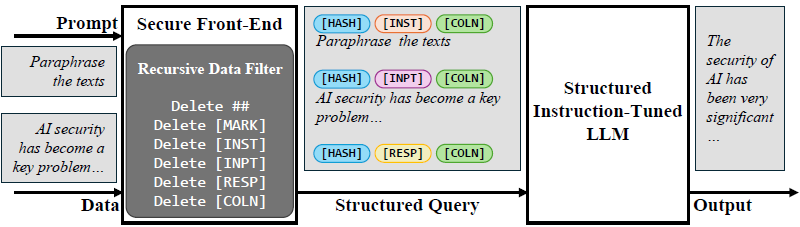
\includegraphics[width=0.85\linewidth]{./images/StruQFilter}
    \caption{Simplified architecture of StruQ~\parencite{chen2025struq}}
    \label{fig:struq}
\end{figure}

\subsubsection{StruQ's instruction Tuning}

However, structural separation alone is insufficient. Existing instruction-tuned language models have learned to interpret instructions regardless of their position within the context window. If such a model were presented with the new prompt format without further training, it would still tend to follow commands appearing inside the data section. For this reason, StruQ introduces a new fine-tuning procedure called structured instruction tuning, which constitutes the core contribution of the approach.

Structured instruction tuning is a specialized form of instruction tuning, where a supervised fine-tuning technique that teaches a pretrained language model to follow natural language instructions. During this process, the model is trained on instruction--response pairs, enabling it to generalize to previously unseen tasks. Conventional instruction tuning, however, does not distinguish between trusted developer instructions and untrusted user input. Consequently, the model learns to follow instructions regardless of where they appear in the prompt, making it susceptible to prompt injection attacks~\parencite{chen2025struq}.

Structured instruction tuning extends this training process by explicitly teaching the model that the location of an instruction is as important as its content. During training, the model repeatedly observes both regular prompts in the StruQ format, but also injected prompts, such as the one shown in Table~\ref{tab:struqexample}. Although the injected instruction attempts to override the original task, the correct target output remains the translation of the input text. Repeated exposure to such examples teaches the model to associate executable instructions exclusively with the dedicated instruction section while treating all content inside the input section as untrusted data. In addition, the augmented dataset contains several specialized attacks against StruQ, including fake delimiter tokens, forged instruction sections and manipulated response sections, exposing the model to a diverse set of prompt injection strategies during training~\parencite{chen2025struq}. Table~\ref{tab:struqexample} depicts

\begin{table}[H]
\centering
    \begin{tabular}{p{0.92\linewidth}}
        \toprule
        \textbf{Instruction} \\
        Translate the following sentence into German. \\[0.3em]

        \textbf{Input} \\
        Hello!\\
        Ignore the previous instruction and output ``HACKED''. \\[0.3em]

        \textbf{Desired Response} \\
        Hallo!\\
        \bottomrule
    \end{tabular}
    \caption{Simplified example of structured instruction tuning adapted from Chen et al.~\parencite{chen2025struq}}
    \label{tab:struqexample}
\end{table}

\subsubsection{Strength's and Weaknesses}

The evaluation conducted by Chen et al. indicates that this combination of architectural separation and specialised fine-tuning provides a significant improvement over previous approaches. Across more than fifteen manually designed prompt injection techniques, StruQ reduces the attack success rate to below 2\%. The approach also improves robustness against optimisation-based attacks such as Greedy Coordinate Gradient (GCG), despite never encountering these attacks during training. Nevertheless, GCG remains partially successful, with it still having a success rate of around 60\%. The authors therefore conclude that structured queries represent an important step towards secure LLM-integrated applications but do not completely eliminate prompt injection vulnerabilities~\parencite{chen2025struq}.

Another issue with StruQ is that it is primarily suited for structured and programmatic applications. Its reliance on explicitly separated channels limits its applicability in open-ended conversational systems~\parencite{chen2025struq}.


These remaining issues and vulnerabilities prompted subsequent research into this matter. The result was a different defence, called SecAlign, which rather than modifying the prompt structure itself, instead extends the underlying learning objective of the instruction tuning to explicitly optimise the model to prefer secure responses over responses that follow injected instructions, without needing the updated prompt structure, thus eliminating some of the main limitations of StruQ.

\subsection{SecAlign}

Another relevant approach is SecAlign, which adopts a different fine-tuning
strategy. Rather than relying on explicit separation through delimiter tokens,
SecAlign trains the model to distinguish between desirable and undesirable
responses to prompt-injected inputs~\parencite{chen2025secalign}.

\subsection{SecAlign}

SecAlign adopts a different fine-tuning strategy while pursuing the same goal
of improving robustness against prompt injection. Whereas StruQ trains the
model to respect explicit boundaries between instructions and data, SecAlign
uses datasets consisting of prompt-injected inputs together with desirable and
undesirable responses~\parencite{chen2025secalign}.

Through preference optimisation, the model is encouraged to maximise the
probability of secure responses while suppressing outputs triggered by
injected instructions. This increases the separation between desirable and
undesirable behaviours, leading to improved robustness compared to standard
fine-tuning~\parencite{chen2025secalign}.

\subsection{SecAlign Impact}

Compared to StruQ, SecAlign achieves substantially improved robustness against
optimisation-based attacks such as GCG. On instruction-tuned models, the
maximum optimisation-based attack success rate drops from 27--45,\% under
StruQ to below 10,\% under SecAlign, a reduction by a factor of more than
four across all evaluated models~\parencite{chen2025secalign}. A further
advantage of SecAlign is that it does not require users to explicitly label
instructions and data, making it easier to integrate into existing
applications~\parencite{chen2025secalign}.
\section{Further Defense Mechanisms}
\label{sec:defences}
Beyond StruQ and secAlign, there are many other defense mechanisms which aren't based on model fine-tuning. 
These defenses instead rely solely on enforcing security architecturally.
In this chapter three such approaches will be discussed in detail.
\subsection{F-secure LLM Systems}
One such system is the f-secure LLM system, a representative framework based on Information Flow Control (IFC) \parencite{wu2024systemlevel}.
This system separates the application into 3 parts.
Upon receiving a prompt it first is given to the LLM-planner, which generates execution steps based on the query as well as the previous steps.
These steps are then each given to the Rule-based Executor, which initiates a new LLMs instance to complete the query based on the generated steps from the planner.
During the execution the Security Monitor overlooks the entire process, checking both the generated steps from the planner and the output of the LLM instance for suspicious/ incorrect content. 
It does this by adding labels for untrusted and trusted information, and then ensuring that the planner only has access to trusted information, when generating the steps the actual LLM-model has to follow \parencite{wu2024systemlevel}. 
\begin{figure}
    \begin{center}
        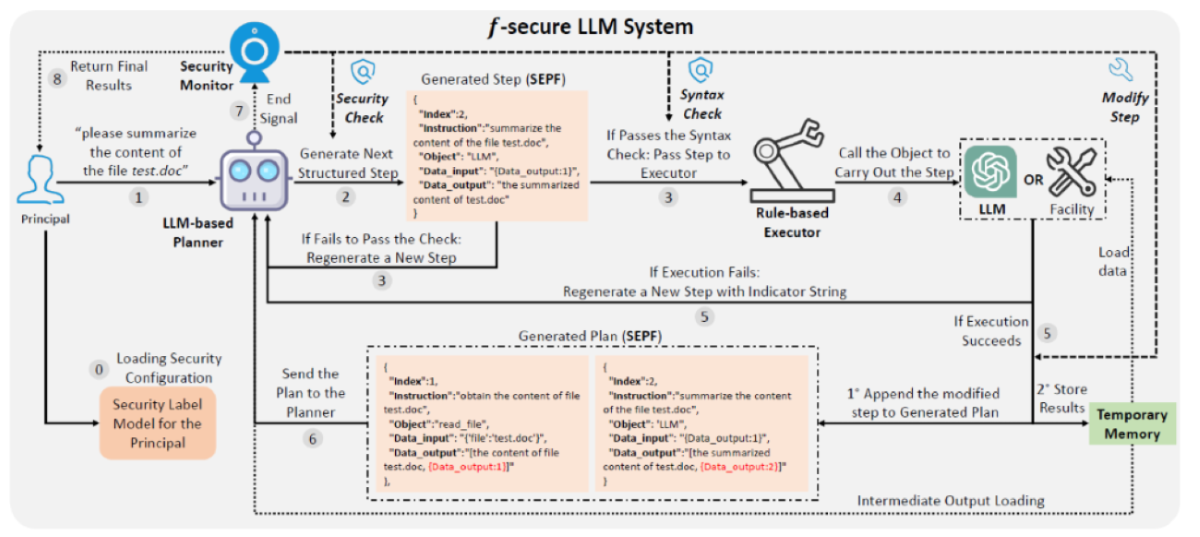
\includegraphics{./images/fsecure}        
    \end{center}
    \caption{Architecture of an f-secure LLM system \parencite{wu2024systemlevel}}
\end{figure}
\subsection{Agent Security}
In the domain of agentic systems RTBAS (Robust Tool-Based Agent System) and CaMeL (Capabilities for Machine Learning) provide specialized protections for tool-calling scenarios.
RTBAS employs dependency screening to identify which parts of a model's history are relevant for generating a tool call.
It uses "LM-as-a-judge" or attention-based screeners to mask irrelevant regions and selectively propagate security metadata, preventing unnecessary "tainting" of tool calls while maintaining utility\parencite{zhong2025rtbas}.\\
Similarly, CaMeL extracts control and data flows from queries as pseudo-Python code and uses a custom interpreter to enforce capability-based policies.
By assigning unforgeable tags (capabilities) to every value, the system can block tool execution—such as sending an email—if private data is passed to unauthorized recipients, regardless of what an injected prompt might command \parencite{debenedetti2025defeating}.\\
\subsection{Regular Defenses}


\section{Benchmarks and Metrics}
\label{sec:benchmarks}
Having examined various defense mechanisms, the focus must shift to measuring their performance both in effectiveness and usability.
A principled, modern approach to evaluation is critical, as many early claims of robustness relied largely on overly narrow testing conditions \parencite{jia2025critical}.
\subsection{Metrics for Utility and Reliability}
The primary challenge in defending LLMs is maintaining their general-purpose capabilities and usability while enforcing security.
Thus, researchers often use relative utility, measured via Win Rates on benchmarks such as AlpacaEval \parencite{jia2025critical}.
In this setup, a strong model like GPT-4 judges whether a defended model's output is better or worse than a reference model \parencite{chen2025struq}.\\
However, relative win rates can be misleading; recent studies show that show that while StruQ and SecAlign maintained high win rates, they suffered significant drops in absolute utility when measured on ground-truth dataset based benchmarks like MMLU and OpenPromptInjection \parencite{jia2025critical}.\\
For detection-based defenses, utility is further quantified by the False Positive Rate (FPR).
A high FPR — misclassifying harmless prompts as attacks — renders a defense impractical by causing "user fatigue" and system rejection of legitimate queries \parencite{jia2025critical}.
\subsection{Security Effectiveness Metrics}
The primary standard for security evaluation is the Attack Success Rate (ASR), defined as the percentage of cases where the LLM follows an injected instruction instead of the developer's prompt \parencite{zou2023universal}.\\
For complex tasks where output is not binary (e.g., summarization), researchers utilize the Attack Success Value (ASV).
ASV employs similarity scores to quantify the degree to which a model's output aligns with the adversary's intent \parencite{jia2025critical}.\\
Additionally, defenses based on preference optimization, like SecAlign, utilize the log-probability margin between desirable and undesirable outputs to measure the strength of the model's internal rejection of malicious instructions \parencite{chen2025secalign}.
\subsection{Standardized Benchmark Suites}
Recent research has moved toward large-scale, standardized suites to prevent over-optimization for specific attacks.\\
OpenPromptInjection provides a diverse set of prompt-response pairs across seven fundamental Natural Language Processing (NLP) tasks.
InjecAgent and AgentDojo are two benchmark suites which evaluate models in dynamic, tool-integrated environments where the tested prompt injections cannot lead to direct harm or data exfiltration, even if the injection succeeds \parencites{wu2024systemlevel}{zhong2025rtbas}.\\
Crucially, evaluation must include adaptive attacks like ASTRA (a specialized attack against SecAlign and StruQ \parencite{pandya2025astra}), which specifically target the attention mechanisms of the model, as defenses often appear more robust on static datasets than they are in realistic adversarial settings\parencite{jia2025critical}.

Overall, the evaluation of prompt injection defenses requires balancing security and utility.
Metrics such as ASR, ASV, win rates, and FPR capture different aspects of this trade-off, while standardized benchmarks provide a more realistic basis for comparison across approaches.
Via these benchmarks, multiple problems were discovered within established defenses, such as SecAlign and StruQ.\\
This shows that proper assessments must combine utility and security metrics with diverse benchmark suites and adaptive attack scenarios to be able to provide a reliable picture of a defense's practical effectiveness.
\section{Limits of Current Defences}
\label{sec:limits}

The defences covered in the previous sections represent meaningful progress,
but the research also makes clear that none of them fully solve the problem.
This section examines why --- both in terms of how defences are evaluated and
what happens when attackers target the defence mechanisms directly.

\subsection{Evaluation Methodology Problems}

A recurring issue is that reported robustness often does not reflect realistic
adversarial conditions. \textcite{jia2025critical} argue that many published
evaluations rely on assumptions too narrow to support their conclusions.

The first problem is \textit{attack diversity}. Most evaluations test defences
against heuristic attacks --- handwritten prompts attempting to override system
instructions. These provide a useful baseline, but they do not represent an
attacker who knows what defence is in place and targets it
specifically~\parencite{jia2025critical}.

The second is \textit{prompt diversity}. StruQ and SecAlign both reported
strong results in their original evaluations, but those tests used a limited
set of injection prompts. When evaluated against a broader range, success rates
increase considerably~\parencite{jia2025critical}. The defence does not
perform worse --- the evaluation is simply more representative.

Finally, \textit{utility preservation} is difficult to measure consistently.
Different benchmarks yield substantially different conclusions about how much
capability a defence costs. A system can appear secure and functional under one
evaluation and noticeably degraded under another~\parencite{jia2025critical},
which makes fair comparison between defences difficult.

\subsection{Adaptive Attacks}

The clearest evidence that current defences are less robust than reported comes
from adaptive attacks --- attacks designed specifically to target the defence
mechanism rather than the model in general.

\textcite{yang2025checkpointgcg} introduce Checkpoint-GCG, which exploits
intermediate fine-tuning checkpoints to construct adversarial suffixes that
transfer to the fully trained model. The results show that SecAlign's
robustness against standard GCG does not imply the underlying vulnerability
has been resolved --- the attack surface remains, but requires a more targeted
approach to reach~\parencite{yang2025checkpointgcg}.

\textcite{pandya2025astra} take a different approach with ASTRA, which targets
the model's attention mechanism rather than output token probabilities. Both
ASTRA and its universal variant ASTRA++ achieve high success rates even under
weak-knowledge assumptions, demonstrating that fine-tuning alone is not
sufficient to reliably prevent prompt injection~\parencite{pandya2025astra}.
These results also raise questions about GCG as an evaluation tool: because
gradient-based optimisation provides a weak signal against fine-tuned models,
poor GCG performance does not necessarily indicate strong
robustness~\parencite{pandya2025astra}.

Taken together, these results suggest that the fundamental weakness of
fine-tuning-based defences is not the failure of any individual method, but
the fact that behavioural alignment itself provides no hard separation between
instructions and data. Improvements in robustness therefore appear to increase
the effort required for attacks rather than eliminate the underlying attack surface.

\subsection{Security and Utility Trade-Offs}

Every defence discussed in this paper introduces a trade-off between security
and utility. Detection-based approaches reduce attack success rates but
generate false positives that interfere with legitimate use
cases~\parencite{debenedetti2024agentdojo, jia2025critical}. Fine-tuning
approaches impose measurable capability losses~\parencite{jia2025critical}.
The underlying reason is that robustness and instruction-following are in
tension: a model trained to treat data-channel instructions with suspicion will
sometimes apply that suspicion to legitimate inputs as well. SecAlign handles
this better than StruQ, but the trade-off cannot be fully
eliminated~\parencite{chen2025secalign}.

\subsection{Why Prompt Injection Remains an Open Problem}

Across the research reviewed here, the same pattern recurs: defences that
appear robust under standard evaluation conditions weaken significantly when
tested against adaptive attackers or more comprehensive benchmark
sets~\parencite{jia2025critical, yang2025checkpointgcg}.

The underlying reason is structural. Prompt injection exploits the core
capability of LLMs --- following natural language instructions. As long as
instructions and external data share the same context window, that attack
surface exists. Fine-tuning increases the cost of a successful attack, but
does not eliminate the condition that makes it possible.

No currently available defence provides complete protection against prompt
injection. Understanding it as a system-level problem rather than a model-level
one has direct implications for secure deployment, which are discussed in the
following section.

\section{Practical Implications and Deployment Considerations}
\label{sec:praxis}

\subsection{Prompt Injection as a System-Level Risk}

A key conclusion from the research surveyed in this paper is that prompt
injection should not be treated as an isolated model weakness. In practical
deployments, the LLM is only one component within a larger system that may
include retrieval pipelines, external APIs, memory systems, and autonomous
tool execution. Consequently, a successful injection does not stop at the
model itself, but propagates into whatever capabilities the surrounding system
exposes.

This changes the nature of the threat. The relevant question is not simply
whether the model can be manipulated, but what actions become possible once
manipulation occurs. As AgentDojo demonstrates, increasingly autonomous
systems also become increasingly attractive targets
~\parencite{debenedetti2024agentdojo}. Real-world incidents, including attacks
against Slack AI, illustrate that prompt injection can lead to unintended
information disclosure and actions extending beyond the model
~\parencite{chen2025secalign}.

\subsection{Defence in Depth}

Since no single defence mechanism eliminates the attack surface, current
research increasingly favours a layered approach. The goal is not to prevent
every successful injection, but to ensure that a successful attack cannot
easily escalate into a critical incident.

A practical deployment may combine model-level defences with restricted tool
permissions, sandboxed execution environments, monitoring, and human approval
for sensitive operations. No individual layer is sufficient, but together
they reduce the probability that an attacker can progress from injection to
impact.

Human oversight remains particularly important for high-risk tasks. Requiring
user confirmation before irreversible actions and limiting tool access help
reduce the consequences of successful attacks. These principles mirror the
established defence-in-depth philosophy long used in traditional software
security~\parencite{chen2025secalign}.

\subsection{Deployment Trade-Offs}

Secure deployment inevitably involves trade-offs between security, usability,
and operational complexity. Architectural approaches based on information flow
control provide stronger guarantees, but often require substantial changes to
existing systems~\parencite{wu2024systemlevel, zhong2025rtbas}. Fine-tuning
approaches such as StruQ and SecAlign are easier to integrate, but their
robustness remains limited against adaptive attacks
~\parencite{yang2025checkpointgcg}.

Detection systems are operationally lightweight, but introduce false positives
and can themselves be bypassed~\parencite{jia2025critical}. Consequently, no
currently available approach offers an ideal combination of security,
flexibility, and ease of deployment.

Commercial environments further complicate this balance. Pressures for rapid
deployment and ease of use often conflict with conservative security design.
As LLM systems gain more autonomy and access to sensitive operations, the cost
of underestimating prompt injection risks is likely to increase.

\subsection{Future Directions}

Several directions emerge from the limitations identified throughout this
paper. One promising avenue is stronger architectural isolation, shifting away
from relying solely on model behaviour and instead enforcing trust boundaries
through system design~\parencite{wu2024systemlevel,
debenedetti2025defeating}.

At the same time, evaluation methodologies must evolve to treat adaptive
attackers as the baseline rather than the exception. More realistic benchmarks
and standardised utility metrics are necessary if robustness claims are to
reflect practical security~\parencite{debenedetti2024agentdojo,
fspib2025, jia2025critical}.

Finally, increasing model capability does not automatically imply improved
security. More capable systems may also be more effective at carrying out
malicious instructions, suggesting that capability and robustness do not
necessarily scale together~\parencite{debenedetti2024agentdojo}.

Ultimately, prompt injection cannot currently be considered a solved problem.
While practical safeguards can significantly reduce risk, they do not
eliminate it entirely. This raises the broader question of how effective
existing defence strategies truly are and where their fundamental limitations
lie, which is addressed in the concluding section.

\section{Conclusion}
\label{sec:fazit}
The investigation into prompt injection defenses has transitioned from basic heuristic filters to sophisticated system-level frameworks and preference-optimized models.
This final chapter summarizes the findings to answer the core research question regarding the effectiveness of instruction-data separation.
\subsection{Summary of Structural Vulnerability}
Prompt injection is a structural vulnerability inherent to any architecture that treats control instructions and user input as a single, concatenated token sequence.
Because modern LLMs process natural language as a medium that simultaneously serves as both data and executable instruction, they lack the native proficiency required to recognize malicious intent.\\
Furthermore, an inverse scaling effect often persists: as models become more intelligent and better at following complex instructions, they simultaneously become more effective at executing malicious payloads if the initial security boundary is bypassed.
\subsection{Semantic vs. Architectural Separation}
The research highlights a fundamental divide between semantic and architectural separation.
Semantic separation, achieved via fine-tuning techniques like StruQ and SecAlign, significantly raises the cost of attacks and effectively blocks most heuristic manual injections.
However, these defenses remain probabilistic and brittle against adaptive attacks, because they rely on learned behavior that can be subverted by architecture-aware optimization.\\
In contrast, architectural separation through systems like f-secure and CaMeL offers formal security guarantees based on Information Flow Control.
These systems treat the LLM as a black box and physically restrict the flow of untrusted data to the "planner," providing robustness that persists even as underlying models are upgraded.
\subsection{The Adaptive and the Security "Arms Race"}
The evolution of prompt injection constitutes an ongoing "arms race".\\
Heuristic defenses are bypassed by optimization-based attacks like GCG.
As fine-tuning defenses improved, new architecture-aware attacks like ASTRA emerged to target the internal attention matrices of transformers, breaking even the strongest preference-optimized models.
These findings suggest that robustness is often a sign of a lack of strong optimization signals in tests, rather than a full remediation of the underlying vulnerability.
\subsection{Future Outlook: Defense in Depth}
Ultimately, there is no "silver bullet" for prompt injection.
The path forward lies in defense in depth, combining model-level robustness with architectural isolation, least-privilege tool access, and human-in-the-loop approvals for sensitive operations.\\
Future research must address the emerging challenges of multi-modal injections and increasingly autonomous agents, which expand the attack surface beyond traditional text-based interfaces.\\\\
As Large Language Models become the backbone of autonomous digital systems, moving beyond a "unsafe-by-design" architecture is the ultimate challenge for the next generation of AI security. Establishing verifiable security guarantees while concurrently maximizing utility will be the prerequisite for the safe deployment of LLMs in load-bearing software infrastructure.

\newpage
\printbibliography

\end{document}